\documentclass[11pt,a4paper]{article}
\usepackage[margin=1in]{geometry}
\usepackage{amsmath,amssymb,booktabs,graphicx,float,caption,hyperref,setspace}
\hypersetup{colorlinks=true,linkcolor=blue,urlcolor=blue,citecolor=blue}
\setstretch{1.1}
\title{\textbf{AQI Analysis and Prediction Across 26 Indian Cities:\\A From-Scratch Data Science Pipeline}}
\author{Vibhuti Negi \and Eashan Vashisht}
\date{\today}
\begin{document}
\maketitle

\begin{abstract}
Air quality in India varies strongly with city and season. This project analyses the Kaggle \emph{Air Quality Data in India (2015--2020)} dataset, covering 24{,}850 city-days from 26 cities, and predicts the Air Quality Index (AQI) from pollutant readings. We build a complete pipeline: SQL-based ingestion, cleaning, descriptive and inferential statistics, feature engineering, forward feature selection, PCA, and linear regression solved in four ways (normal equation, gradient descent, ridge regression and random search). All statistics and models are implemented from formulas rather than library routines. On a time-ordered test set the models reach $R^2\approx0.77$ and RMSE $\approx 42.8$. We discuss why the error is dominated by a few extreme cities and the limits of a single linear model.
\end{abstract}

\section{Introduction}
\subsection{Problem statement}
The Air Quality Index condenses several pollutant concentrations into one number, but it differs sharply between cities and across seasons. Understanding which pollutants and conditions drive AQI, and predicting it for future days, supports public health decisions.

\subsection{Objectives}
\begin{enumerate}
\item Profile and clean the multi-city pollutant dataset.
\item Test statistically whether season and city explain differences in AQI.
\item Engineer and select features that predict AQI.
\item Implement linear regression from scratch with several optimisation methods.
\item Evaluate the models on unseen future dates and interpret their limits.
\end{enumerate}

\subsection{Scope}
All 26 cities in the dataset, daily readings from January 2015 to July 2020, tabular regression only (no deep learning, no weather data).

\section{Dataset}
\subsection{Source}
The data is the public Kaggle dataset \emph{Air Quality Data in India (2015--2020)} \cite{kaggle}, file \texttt{city\_day.csv}, compiled from Central Pollution Control Board (CPCB) records. It has 29{,}531 rows; 24{,}850 rows contain an AQI value and form our working set. No duplicate (City, Date) pairs exist.

\subsection{Attributes}
\begin{table}[H]
\centering
\begin{tabular}{@{}lll@{}}
\toprule
Group & Columns & Type \\ \midrule
Particulates & PM$_{2.5}$, PM$_{10}$ & float64 ($\mu$g/m$^3$) \\
Gases & NO, NO$_2$, NO$_x$, NH$_3$, CO, SO$_2$, O$_3$ & float64 \\
VOCs & Benzene, Toluene, Xylene & float64 \\
Target & AQI & float64 \\
Keys & City, Date & object, datetime64 \\ \bottomrule
\end{tabular}
\caption{Structure of \texttt{city\_day.csv}. \texttt{AQI\_Bucket} is a label derived from AQI and was removed to avoid leakage.}
\end{table}

\section{Methodology}
\subsection{Pipeline}
We follow the CRISP-DM stages \cite{crisp}: data understanding, preparation, modelling and evaluation. The CSV is read in chunks of 5{,}000 rows (batch ingestion), loaded into an in-memory SQLite table (a small warehouse) and queried with SQL to keep rows where AQI is not null.

\subsection{Cleaning}
\begin{table}[H]
\centering
\begin{tabular}{@{}lll@{}}
\toprule
Issue & Finding & Decision \\ \midrule
Missing target & AQI blank on 16\% of rows & Rows dropped \\
Heavy missing & Xylene 61.9\% & Column dropped (threshold 35\%) \\
Moderate missing & PM$_{10}$ 28.5\%, NH$_3$ 26.3\%, Toluene 23.4\% & Median of the same city \\
Light missing & Benzene 14.2\%, NO$_x$ 7.5\%, others $<4\%$ & Median of the same city \\
Outliers & Right-skewed spikes & Clip at $Q_1-3\,\mathrm{IQR}$, $Q_3+3\,\mathrm{IQR}$ \\
Types & Date stored as text & Converted to datetime, sorted \\ \bottomrule
\end{tabular}
\caption{Cleaning decisions. After cleaning no missing values remain.}
\end{table}
The target is never imputed, since imputing it would invent labels. City-wise medians are used because pollution levels differ greatly between cities, so a global median would distort local readings.

\subsection{Statistical methods}
All formulas below were coded by hand. For a sample $x_1,\dots,x_n$:
\begin{align}
\bar{x} &= \frac1n\sum_i x_i, \qquad s^2=\frac{1}{n-1}\sum_i (x_i-\bar x)^2,\\
\text{skew} &= \frac1n\sum_i\left(\frac{x_i-\bar x}{s}\right)^3, \qquad
r_{xy}=\frac{\sum_i (x_i-\bar x)(y_i-\bar y)}{\sqrt{\sum_i (x_i-\bar x)^2\sum_i (y_i-\bar y)^2}}.
\end{align}
\textbf{Welch t-test} \cite{welch} for winter (W) versus monsoon (M), one-tailed with $H_1:\mu_W>\mu_M$:
\begin{equation}
t=\frac{\bar x_W-\bar x_M}{\sqrt{s_W^2/n_W+s_M^2/n_M}}.
\end{equation}
\textbf{One-way ANOVA} over $k$ groups with $N$ observations:
\begin{equation}
F=\frac{SS_B/(k-1)}{SS_W/(N-k)},\quad SS_B=\sum_g n_g(\bar x_g-\bar x)^2,\quad SS_W=\sum_g\sum_i (x_{gi}-\bar x_g)^2.
\end{equation}
A two-way ANOVA with factors Season and Period (before 2020 versus 2020) divides each factor's sum of squares by its degrees of freedom and by the within-cell mean square. A chi-square test checks whether observations are equally spread across seasons, $\chi^2=\sum (O-E)^2/E$. The central limit theorem is verified by drawing 2{,}000 samples of size 30 and comparing the standard deviation of the sample means with $\sigma/\sqrt{30}$.

\subsection{Feature engineering and selection}
New features: PM ratio $=\mathrm{PM}_{2.5}/\mathrm{PM}_{10}$, $\log(1+\mathrm{CO})$, $\mathrm{NO}_x-\mathrm{NO}_2$, a winter indicator, a cyclic month encoding $(\sin\frac{2\pi m}{12},\cos\frac{2\pi m}{12})$, a per-city one-day lag of PM$_{2.5}$, and one-hot city indicators (25 dummies, one city as reference).

A filter step keeps numeric features with $|r|>0.2$ against AQI (13 of 18 pass). A wrapper step then applies \emph{forward selection}: starting from an empty set, add the feature that most increases validation $R^2$, for eight steps. Features are standardised, $z=(x-\mu_{\text{train}})/\sigma_{\text{train}}$, with training statistics only, to avoid leakage.

PCA is computed from the eigen-decomposition of the covariance matrix $\Sigma$ of the standardised numeric features: $\Sigma v_j=\lambda_j v_j$, with explained variance ratio $\lambda_j/\sum_k\lambda_k$.

\subsection{Models and optimisation}
With design matrix $X$ (bias column included) and target $y$, the cost is
\begin{equation}
J(\theta)=\frac{1}{2m}\lVert X\theta-y\rVert^2 .
\end{equation}
Four solvers minimise it:
\begin{align}
\text{Normal equation:}&\quad \theta=(X^\top X)^{-1}X^\top y,\\
\text{Gradient descent:}&\quad \theta\leftarrow\theta-\frac{\alpha}{m}X^\top(X\theta-y),\\
\text{Ridge \cite{ridge}:}&\quad \theta\leftarrow\theta-\frac{\alpha}{m}\left[X^\top(X\theta-y)+\lambda\theta_{1:}\right],
\end{align}
and a non-gradient \emph{random search}, which perturbs $\theta$ with Gaussian noise and keeps the change when the loss falls. Settings: $\alpha=0.1$, 800 epochs, $\lambda=20$, 12{,}000 random-search iterations with a step size shrinking by a factor 0.4 every 3{,}000 iterations. At the optimum the gradient must vanish (necessary condition), which we verify numerically.

\subsection{Train/test split and metrics}
Data is sorted by date and split in time: the first 80\% (2015-01-01 to 2019-12-06) trains, the last 20\% (2019-12-06 to 2020-07-01) tests. A random split would let the model see future days. Metrics:
\begin{align}
\mathrm{RMSE}&=\sqrt{\tfrac1n\sum(y_i-\hat y_i)^2}, \quad \mathrm{MAE}=\tfrac1n\sum|y_i-\hat y_i|,\\
R^2&=1-\frac{\sum(y_i-\hat y_i)^2}{\sum(y_i-\bar y)^2},\quad
R^2_{\text{adj}}=1-(1-R^2)\frac{n-1}{n-p-1}.
\end{align}

\section{Results and Discussion}
\subsection{Descriptive statistics}
\begin{table}[H]
\centering
\begin{tabular}{@{}lrrrr@{}}
\toprule
Variable & Mean & Std & Skewness & Kurtosis \\ \midrule
PM$_{2.5}$ & 64.8 & 51.9 & 1.64 & 5.32 \\
PM$_{10}$ & 111.6 & 72.0 & 1.53 & 5.58 \\
NO$_2$ & 28.4 & 22.6 & 1.59 & 5.79 \\
CO & 1.2 & 1.0 & 1.64 & 5.15 \\
AQI & 166.5 & 140.7 & 3.40 & 24.42 \\ \bottomrule
\end{tabular}
\caption{Descriptive statistics after cleaning.}
\end{table}
All variables are right-skewed, AQI most strongly. Ahmedabad is the most polluted city (mean AQI 452), followed by Delhi (259) and Patna (241); the cleanest are Aizawl (35), Shillong (54) and Coimbatore (73).

\subsection{Hypothesis tests}
\begin{table}[H]
\centering
\begin{tabular}{@{}lll@{}}
\toprule
Test & Statistic & Conclusion \\ \midrule
One-tailed Welch $t$ (winter $>$ monsoon) & $t=49.46$, $p\approx0$ & Reject $H_0$ \\
One-way ANOVA, season & $F(2,24847)=1317.6$ & Season matters \\
One-way ANOVA, city & $F(25,24824)=677.6$ & City matters \\
Two-way ANOVA & $F_{\text{season}}=1381.5$, $F_{\text{period}}=883.0$ & Both significant \\
Chi-square, equal seasons & $\chi^2=2126.7$ (crit. 5.99) & Not equal \\
CLT check & $25.99$ vs $\sigma/\sqrt{n}=25.69$ & Consistent \\ \bottomrule
\end{tabular}
\caption{Inferential results.}
\end{table}
Also, $P(\text{AQI}>300)=0.148$ overall but $0.291$ in winter, so extreme pollution is about twice as likely in winter. The $p$-values use a normal approximation, which is acceptable for $n\approx 25{,}000$; $F$ and $\chi^2$ are compared with tabulated critical values.

\subsection{Feature selection and PCA}
\begin{table}[H]
\centering
\begin{tabular}{@{}clc@{}}
\toprule
Step & Feature added & Validation $R^2$ \\ \midrule
1 & PM$_{2.5}$ & 0.384 \\ 2 & CO & 0.665 \\ 3 & $\log$CO & 0.716 \\ 4 & NO$_2$ & 0.750 \\
5 & NO & 0.757 \\ 6 & PM$_{2.5}$ lag-1 & 0.763 \\ 7 & PM$_{10}$ & 0.765 \\ 8 & Thiruvananthapuram & 0.767 \\ \bottomrule
\end{tabular}
\caption{Forward selection. Gains flatten after step 4.}
\end{table}
The first three principal components explain 39.8\%, 14.6\% and 10.2\% of the variance (64.7\% cumulative), so the pollutants are correlated but not reducible to one or two directions.

\subsection{Model comparison}
\begin{table}[H]
\centering
\begin{tabular}{@{}lcccc@{}}
\toprule
Method & RMSE & MAE & $R^2$ & Adj.\ $R^2$ \\ \midrule
Normal equation & 42.83 & 25.07 & 0.773 & 0.773 \\
Gradient descent & 42.85 & 24.96 & 0.773 & 0.773 \\
Ridge ($\lambda=20$) & 42.87 & 24.95 & 0.773 & 0.773 \\
Random search & 42.80 & 25.04 & 0.774 & 0.773 \\ \bottomrule
\end{tabular}
\caption{Test-set performance. A baseline predicting the training mean scores $R^2=-0.383$.}
\end{table}
All four solvers agree, so the problem is well conditioned, and the norm of the gradient at the normal-equation solution is about $7\times10^{-13}$. Ridge gives no gain, which suggests overfitting is not the issue. The fitted standardised coefficients include PM$_{2.5}$ ($+42.2$), CO ($+156.0$), $\log$CO ($-107.5$), NO$_2$ ($+25.6$) and the lag feature ($+31.2$). The opposite signs of CO and $\log$CO come from their collinearity, so they should be read together. Category accuracy (Good, Satisfactory, Moderate, Poor, Very Poor, Severe) is 66.5\%.

\subsection{Error by city}
Test RMSE is lowest for Aizawl (13.9) and Bengaluru (15.2) and highest for Patna (45.9) and Ahmedabad (151.4). Ahmedabad's very high AQI values dominate the overall error, so one linear model cannot follow every city.

\subsection{Visualisations}
\begin{figure}[H]
\centering
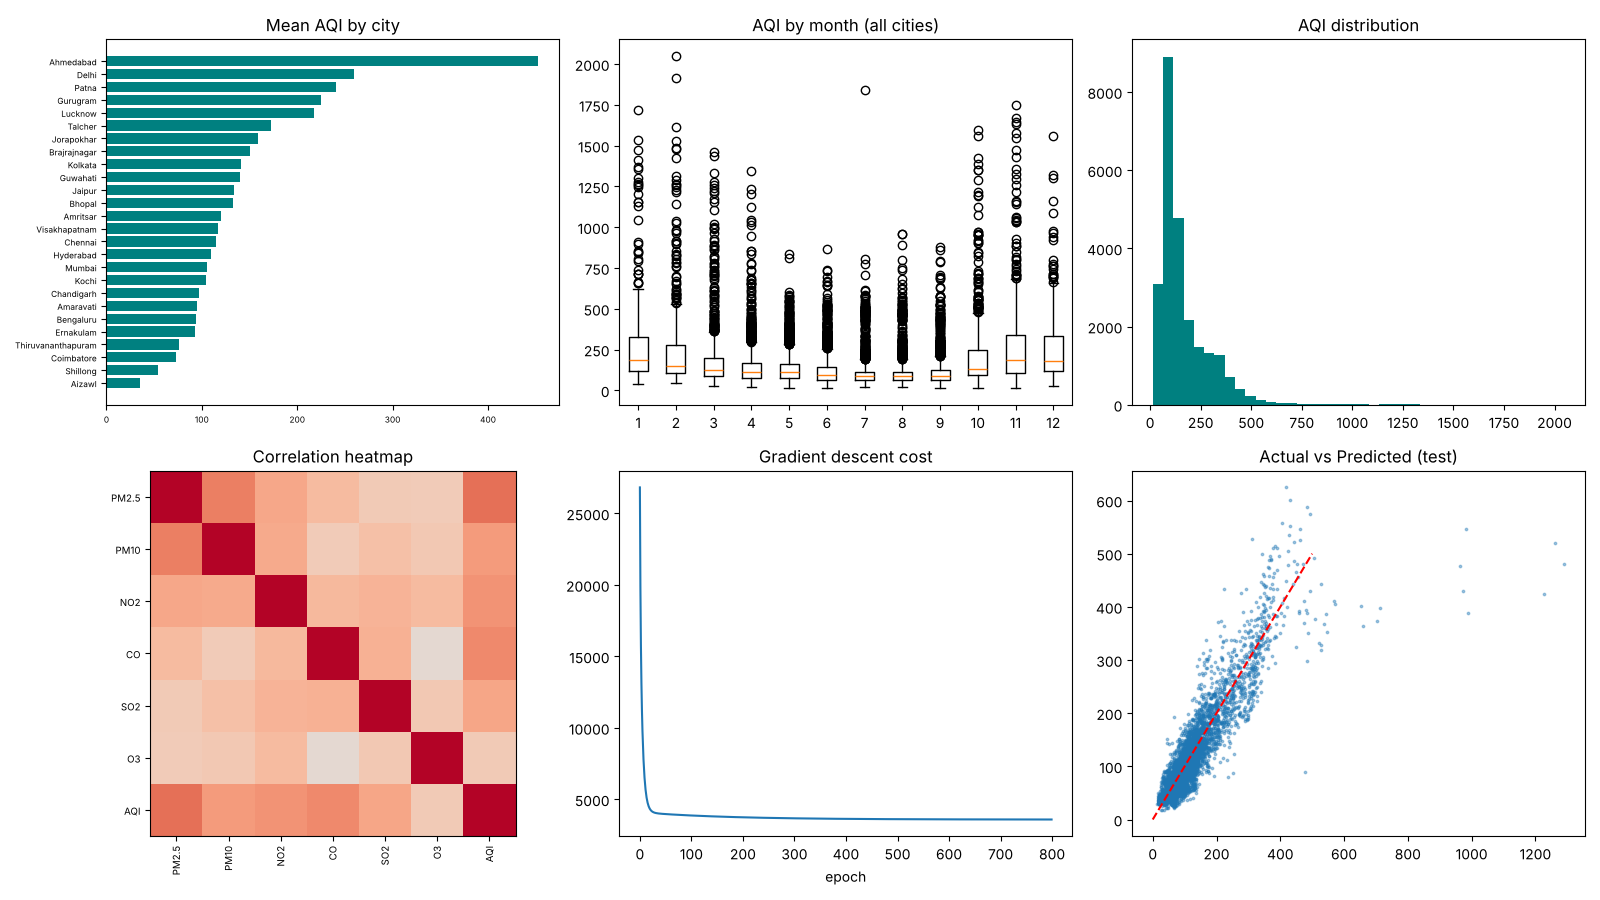
\includegraphics[width=\textwidth]{aqi_plots_all_cities.png}
\caption{Top row: mean AQI by city, AQI by month, AQI histogram. Bottom row: correlation heatmap, gradient descent cost against epochs, actual versus predicted AQI on the test set.}
\end{figure}

\section{Limitations}
\begin{itemize}
\item AQI is computed from pollutant values, so a high $R^2$ is partly expected.
\item The test period (December 2019 to July 2020) differs from the training years and includes the COVID-19 period, which explains the negative baseline $R^2$.
\item Collinear features (CO and $\log$CO, PM$_{2.5}$ and PM$_{10}$) make individual coefficients hard to interpret.
\item A single global linear model cannot capture city-specific behaviour, especially Ahmedabad.
\item $p$-values use a normal approximation and no weather variables are included.
\end{itemize}

\section{Conclusion and Future Work}
We built an end-to-end, formula-based pipeline on 24{,}850 city-days from 26 cities. Winter and city strongly affect AQI, and a linear model on a few pollutant features explains about 77\% of AQI variance on future dates, with all four optimisers converging to the same solution. Future work includes per-city models, time-series models, robust regression for extreme values, and adding weather data.

\begin{thebibliography}{9}
\bibitem{kaggle} R.~Rao, \emph{Air Quality Data in India (2015--2020)}, Kaggle dataset, \url{https://www.kaggle.com/datasets/rohanrao/air-quality-data-in-india}.
\bibitem{crisp} P.~Chapman et al., \emph{CRISP-DM 1.0: Step-by-step data mining guide}, SPSS Inc., 2000.
\bibitem{welch} B.~L. Welch, ``The generalization of Student's problem when several different population variances are involved,'' \emph{Biometrika}, 34(1--2):28--35, 1947.
\bibitem{ridge} A.~E. Hoerl and R.~W. Kennard, ``Ridge regression: biased estimation for nonorthogonal problems,'' \emph{Technometrics}, 12(1):55--67, 1970.
\bibitem{esl} T.~Hastie, R.~Tibshirani and J.~Friedman, \emph{The Elements of Statistical Learning}, 2nd ed., Springer, 2009.
\bibitem{cpcb} Central Pollution Control Board, \emph{National Air Quality Index}, Government of India, 2014.
\end{thebibliography}
\end{document}
